% !TEX output_directory = ./.temp/report
% !TEX options = --shell-escape

\documentclass[a4paper, 12pt]{scrartcl}
\usepackage[assign-num=3]{report}
\usepackage[outputdir=./.temp/report]{minted}
\usepackage{svg}

\title{Comparison of Game Engines}

\begin{document}

\maketitle

\section{Introduction}
A game engine is a tool for developers of video games. It is software framework which abstracts away core parts of a video game such as rendering, physics, input handling, sound, AI, etc. It typically includes software libraries and other software in the form of a software development kit (SDK), which contains additional tools revolving around the engine's ecosystem (level editor, asset packager, and so on).

A game engine enables developers to create games more efficiently, since a lot of the fundamental components of a game are available for use out of the box. This saves developers the time of having to implement all these core features from scratch, which could otherwise add a tremendous amount of complexity to the project. For example, game engines may offer cross-platform capabilities in a more or less transparent way to the developers. This removes the necessity to deal with the plethora of different platform-specific APIs, which allows developers and publishers to reach a broader market more easily.

\subsection{History}
Game engines were not immediately prevalent in the industry when it first started. This is because the platforms were much more fragmented, and there was little standardisation (and thus little compatibility) among them. Furthermore, hardware was being developed at a rapid pace. All these factors made it difficult to re-use any abstractions (such as those provided by a game engine) in the long term. Hardware was also quite limited, so it was necessary to build a game's components from scratch and custom-tailor them to the target platform to ensure the game ran optimally.

The earliest software that may constitute a game engine was in-house for use with first-party software. These engines were far more limited in scope than modern game engines (what may now be considered \textit{middleware} used by a game engine). Engines for third-parties became prevalent in the 1990s along with the growing popularity and feasibility of 3D graphics. This led to influential engines such as id Tech and Unreal Engine, which are in some form or another still in use with modern games.

Such engines were developed for first-party games, but made available for licensing to third-party developers. Companies shifted their strategy to developing the game and its engine separately. This decoupling enabled the engine to be usable by third parties, and allowed developers to become more specialised.

\section{Comparing Source and Unity}
This section compares and contrasts various aspects of two different engines: Source by Valve Software and Unity by Unity Technologies.

\subsection{Development Environment}
\subsubsection{Source}
Programming is done in C++, typically using Visual Studio. However, other IDEs can also work. A level editor named \textit{Hammer} is included in the Source SDK. When not programming or making assets, this is tool that is being worked with the most. It is used to define the level's geometry, apply textures, light the level, place objects and entities, configure behaviour logic for entities, and much more.

\begin{figure}[!htp]
  \centering
  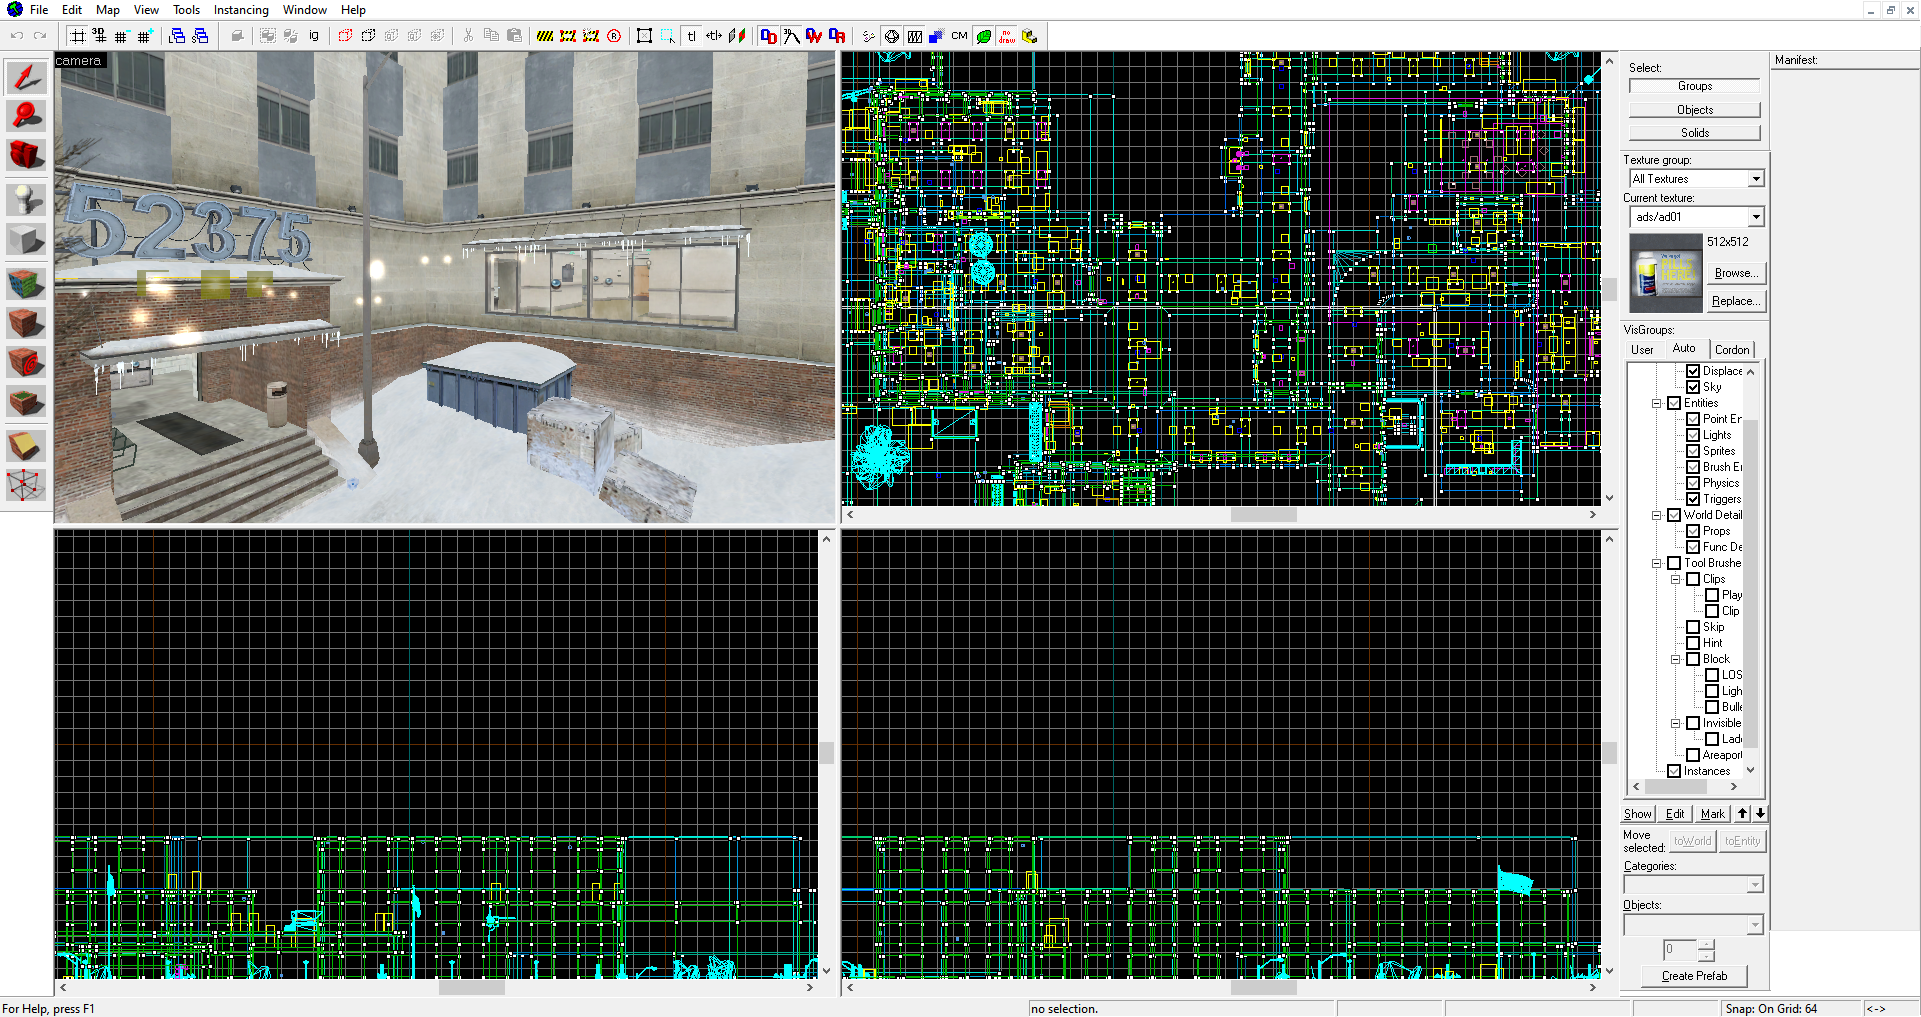
\includegraphics[width=\linewidth]{images/source_hammer.png}
  \caption{Hammer editing \textit{cs\_office} from CS:GO}
\end{figure}

Assets such as models and textures are expected to be created using third-party tools. For modelling, Autodesk XSI and Maya were historically popular. However, it's more common these days to use one of the third-party plugins for other modelling tools such as Blender.

Some assets, including models and textures, are expected to be in Source-specific formats. To achieve this, the Source SDK provides some command-line tools to convert assets to the expected formats. For example, \texttt{vtex} is used for texture conversion and \texttt{studiomdl} is used to compile models. There are various other command-line tools, like \texttt{vbsp}, \texttt{vvis}, and \texttt{vrad} for map compilation and \texttt{vpk} for packaging game assets.

There are also third-party tools frequently used by modders and level designers, such as VIDE, which can be used to create textures, view or create game content packages, edit particles, pack game content into map files, and much more.

\begin{figure}[!htp]
  \centering
  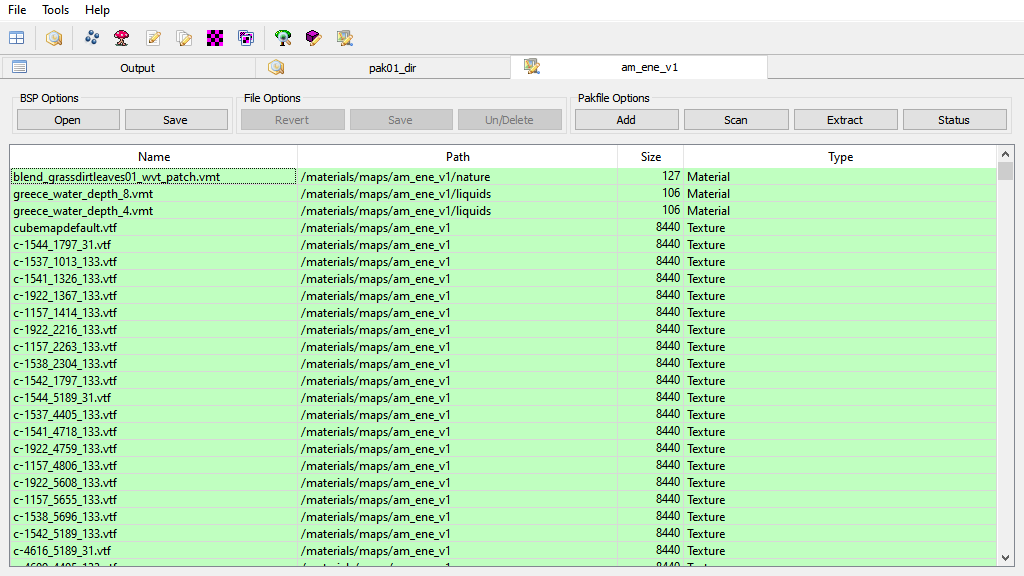
\includegraphics[width=\linewidth]{images/source_vide_pakfile.png}
  \caption{VIDE displaying the pakfile lump of a map}
\end{figure}

\subsubsection{Unity}
The primary development environment for Unity is the Unity Editor. This environment is quite integrated; the Source engine's environment looks dated and fragmented in comparison. Like Hammer, Unity Editor can define the geometry of a scene and apply textures to objects. But it could also do a lot more, like creating animations and materials, running the game within, inspecting a running game's state, designing UIs, creating visual effects, and profiling the game.

\begin{figure}[!htp]
  \centering
  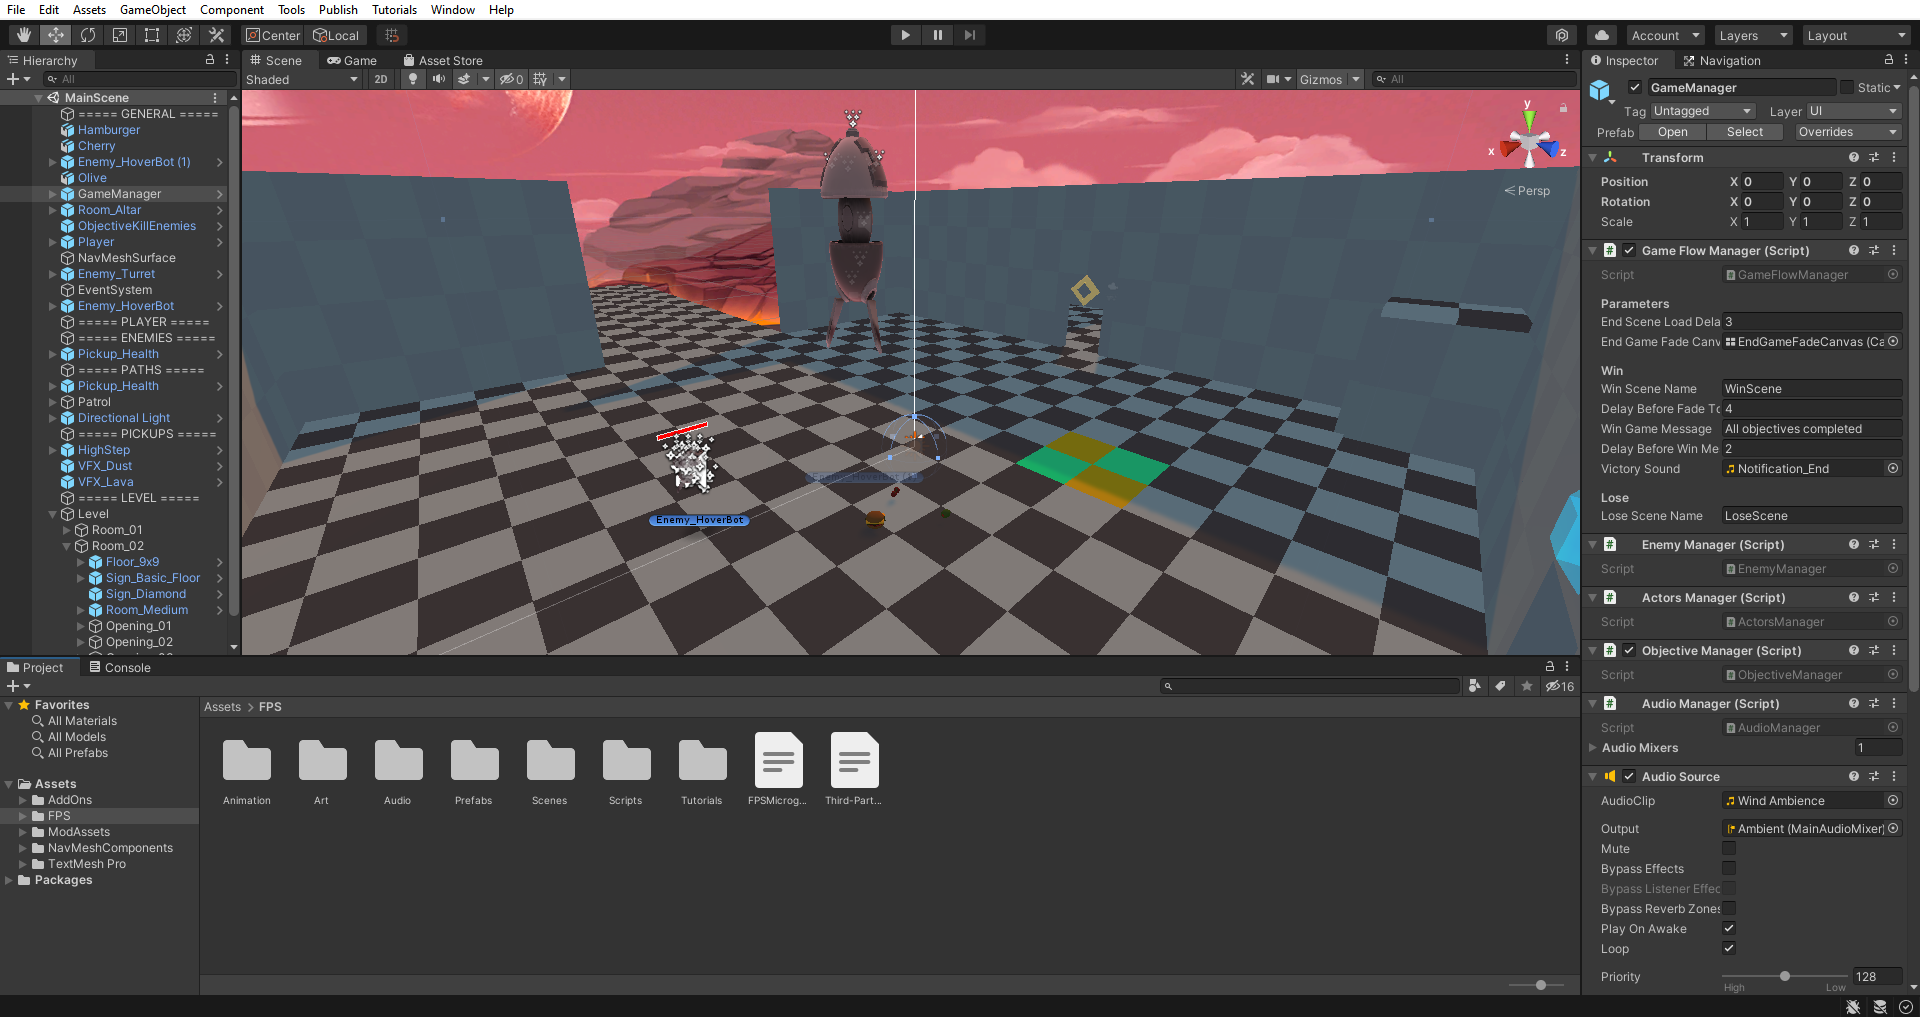
\includegraphics[width=\linewidth]{images/unity_editor.png}
  \caption{Unity Editor}
\end{figure}

The Unity environment is much more extensible than Source. Its package management system makes it easy to obtain first and third-party extensions to the Unity Editor. This same mechanism can also be used to import third-party assets from the internet. In general, using assets is easier compared to Source since Unity supports standard formats, and can even automatically convert formats in some cases.

For scripting, Unity Editor allows scripts to be edited with virtually any text editor. It also natively supports deeper integration with several IDEs: Visual Studio, Visual Studio Code, and JetBrains Rider.

\subsection{Programming}
\subsubsection{Source}
The engine itself is written in C++ so naturally, programming a game with the Source engine is also done in C++. The full source code of the engine can be licensed. Valve also offers a portion of the engine's C++ code with the Source SDK. This is enough to make a game with the SDK, but it doesn't give access to the engine's internals such as its core networking code. The Source engine also comes with it's own Standard Template Library named \texttt{CUtl}, which is located within the \texttt{Tier1} library of the engine.

\paragraph{Scripts}
The engine also supports external scripts using the VScript virtual machine and API. Depending on the version of the SDK, different languages are supported. VScript first shipped with support for the Squirrel language. However, Source Filmmaker uses Python and Portal 2 has limited Lua support.

\begin{figure}[!htp]
  \begin{minted}[
    linenos,
    autogobble=true,
    fontsize=\fontsize{10}{10},
  ]{js}
    function GiveGun(weapon, playerarray) {
      local equipper = Entities.CreateByClassname("game_player_equip")
      equipper.__KeyValueFromInt("spawnflags", 5)
      equipper.__KeyValueFromInt(weapon, 0)
      equipper.ValidateScriptScope()

      for (player in playerarray) {
        EntFireByHandle(equipper, "Use", "", 0, player, null)
      }

      EntFireByHandle(equipper, "Kill", "", 0.1, null, null)
    }
  \end{minted}
  \caption{VScript in Squirrel for CS:GO which equips players}
  \label{fig:source_vscript}
\end{figure}

Scripts can be attached to any entity via the \textit{Entity Scripts} property. Multiple scripts can be attached to an entity simultaneously. The input \texttt{RunScriptCode} can be used to execute VScript code within the script scope of the target entity's attached scripts. Similarly, \texttt{CallScriptFunction} can be used to call a function. There is also \texttt{RunScriptFile}, which can be used to run a script from disk and merge its contents with the script scope of the target entity. Inputs and outputs for entities will be discussed in more detail shortly.

It is technically possible to add support for scripting with any language, without relying on VScript. Garry's mod did this with Lua, and there is also a project by modders which added Python support.

\paragraph{I/O Entities}
Besides directly programming in C++ and VScript, there is an I/O system by which entities communicate between each other. This system can be leveraged to program entities in Hammer. Effectively, an entity's event can be hooked so that an action is performed on another entity when the event occurs.

For example, \cref{fig:source_entities} shows some of the entities used to control an elevator. The four stacked \texttt{logic\_relay}s control the doors for each of the four floors. The \texttt{logic\_compare} chooses the next path node for the elevator to travel to. The \texttt{logic\_relay} at the bottom right performs actions when the elevator needs to stop.

\begin{figure}[!htp]
  \centering
  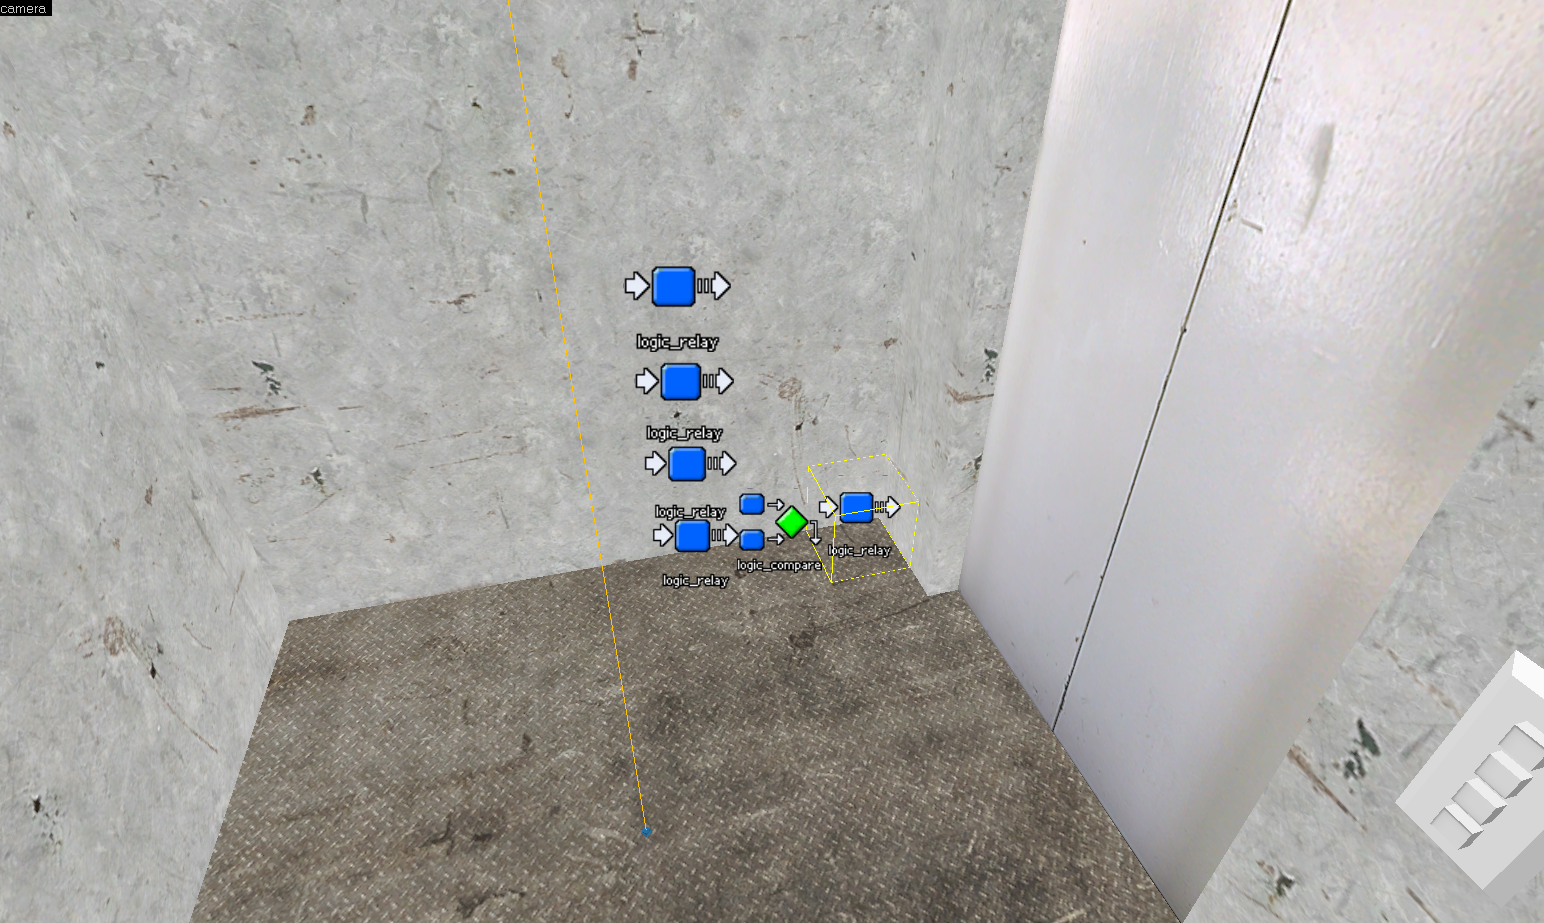
\includegraphics[width=0.75\linewidth]{images/source_io_entities.png}
  \caption{Logic entities for controlling an elevator}
  \label{fig:source_entities}
\end{figure}

The last \texttt{logic\_relay} is pictured in more detail in \cref{fig:source_elev_stop}. The purpose of a \texttt{logic\_relay} is to forward messages; it can turn one input into many outputs. Another entity can trigger the relay, which causes the relay to fire an \texttt{OnTrigger} event. \texttt{elev\_stop} is being triggered by the aforementioned \texttt{logic\_compare}. \texttt{elev\_stop} has four outputs that occur when the \texttt{OnTrigger} event is fired. Each output targets a different entity and sends it some input. The first stops the elevator, the second plays a bell sound, and the last two open doors.

\begin{figure}[!htp]
  \centering
  \subfloat[\centering inputs]{
    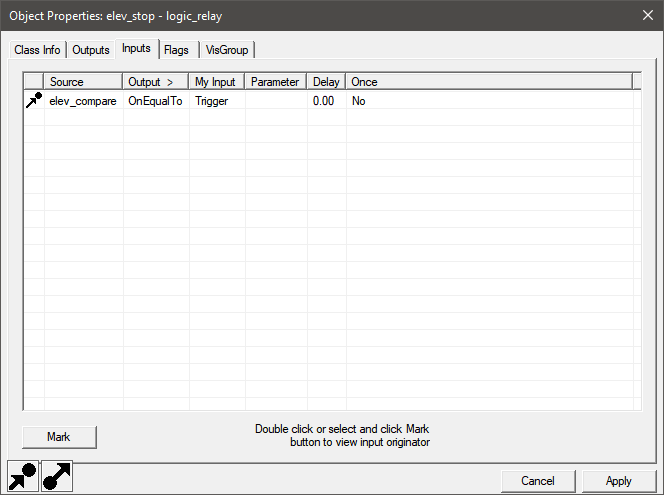
\includegraphics[width=0.45\linewidth]{images/source_io_elev_stop_in.png}
  }
  \qquad
  \subfloat[\centering outputs]{
    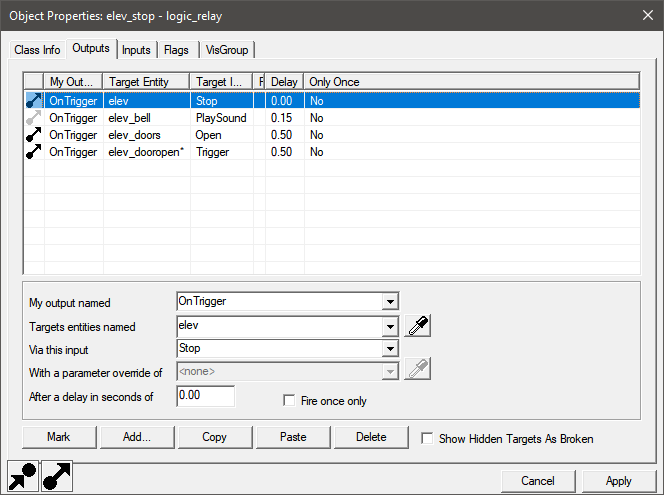
\includegraphics[width=0.45\linewidth]{images/source_io_elev_stop_out.png}
  }
  \caption{The configured I/O of the \texttt{logic\_relay} entity named \texttt{elev\_stop}}
  \label{fig:source_elev_stop}
\end{figure}

\paragraph{Events}
There are many other events, such as one for the player getting hurt or a team winning a round. Data can be associated with an event, for example, which player got hurt or which team won. The \texttt{logic\_eventlistener} entity can be used to listen to events. In C++, \texttt{CGameEventListener::ListenForGameEvent} can be used. The \texttt{CGameEventManager} class can be used to interact with events, be it creating a new event, firing an event, or registering an event listener. Events are declared in various \texttt{.res} files in the \textit{resources} directory of the game. These get loaded using \texttt{CGameEventManager::LoadEventsFromFile}.

\begin{figure}[!htp]
  \begin{minted}[
    linenos,
    autogobble=true,
    fontsize=\fontsize{10}{10},
  ]{js}
    "game_end"              // a game ended
    {
      "winner"  "byte"      // winner team/user id
    }

    "round_start"
    {
      "timelimit" "long"    // round time limit in seconds
      "fraglimit" "long"    // frag limit in seconds
      "objective" "string"  // round objective
    }
  \end{minted}
  \caption{A portion of CS:GO's \textit{resource/gameevents.res}}
  \label{fig:source_gameevents}
\end{figure}

\subsubsection{Unity}
The Unity engine is written in C++. For a fee, it is possible to license the engine's source code and modify it directly. Unlike the Source engine, there is no free offering of a portion of the engine's source code. Thus, for most, the only option is to use Unity's C\# scripting APIs. Thankfully, these APIs are far more powerful and comprehensive than the Source engine's.

\paragraph{Scripts}
Scripts can be attached to game objects as components. This is similar to VScripts in the sense that VScripts can be attached to any entity. The inspector in Unity Editor will show all public fields of the script in the component's UI. There isn't an equivalent to this for VScripts. It's possible to access other scripts' public fields programmatically by getting the script components of other game objects.

\begin{figure}[!htp]
  \centering
  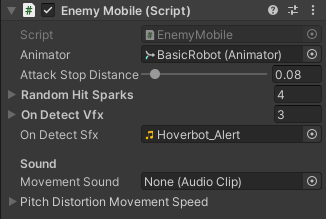
\includegraphics[scale=0.75]{images/unity_script_inspector.png}
  \caption{Setting a script's public fields in the inspector}
  \label{fig:unity_script_inspector}
\end{figure}

Scripts have an \texttt{Update} function which is called every frame. This is similar to the ``think'' function that VScripts have. They also have a \texttt{Start} function which is called before frames start being updated, so it's useful for initialisation code. Neither function has to be used though. For example, it may be desirable to have a script that holds functions used to handle events. Such functions can be hooked up using the inspector.

\begin{figure}[!htp]
  \begin{minted}[
    linenos,
    autogobble=true,
    fontsize=\fontsize{10}{10},
  ]{cs}
    using UnityEngine;

    public class ColourChanger : MonoBehaviour {
        private void Start() {
            Debug.Log("Starting ColourChanger.");
        }

        private void Update() {
            GetComponent<Renderer>().material.color = Random.ColorHSV();
        }
    }
  \end{minted}
  \caption{Script which sets a random colour for the object every frame}
  \label{fig:unity_script}
\end{figure}

\paragraph{Events}
Some events have already been discussed, such as \texttt{Start} and \texttt{Update}. There are many other built-in events, such as UI events (e.g. clicking a button) and physics events (e.g. collision detection).

Custom events can be created using \texttt{UnityEvent} objects. If one is added as a public field of a script, it's possible to add a callback along with an argument for the event via the inspector. This is similar to the outputs menu in Hammer, but with a nicer interface; the editor displays a different UI component depending on the data type of the argument. For example, in \cref{fig:unity_event_inspector}, the argument is represented by a check box since it is a \texttt{bool}.

Alternatively, event listeners can be attached programmatically with \texttt{UnityEvent\-.AddListener}. Events can be invoked programmatically with \texttt{UnityEvent.Invoke}.

\begin{figure}[!htp]
  \centering
  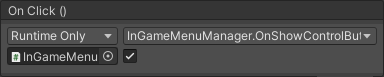
\includegraphics[scale=0.75]{images/unity_event_inspector.png}
  \caption{Attaching a function to a button's \texttt{onClick} event}
  \label{fig:unity_event_inspector}
\end{figure}

There is also a general-purpose messaging system, which can be used to send custom messages to any game object which is registered to receive them. To create a custom message, an interface implementing \texttt{IEventSystemHandler} can be defined with some event handling functions. Then, any game object's script can implement this interface and define concrete event handlers. \texttt{ExecuteEvents.Execute} can be called with a specific \texttt{IEventSystemHandler}, a target game object, and a function in the interface. Any component of the target which implements the interface will have the specified function executed.

\subsection{Input}
\subsubsection{Source}
\subsubsection{Unity}

\subsection{Assets}
\subsubsection{Source}
Assets can be loaded as loose files, from \texttt{vpk} archives, or from the pakfile lumps of \texttt{bsp} files. The Source engine has a multitude of proprietary file formats. The following is a non-comprehensive list of them:

\begin{itemize}
  \item \texttt{ain} -- \textit{\underline{A}rtificial \underline{I}ntelligence \underline{N}odegraph}: the generated node graph used by NPCs for navigation
  \item \texttt{bsp} -- \textit{\underline{B}inary \underline{S}pace \underline{P}artition}: used for game levels/maps
  \item \texttt{mdl} -- \textit{\underline{M}o\underline{d}e\underline{l}}: contains the structure of the model, animations, hit box, materials, mesh, and LOD information
  \item \texttt{nav} -- \textit{\underline{Nav}igation Mesh}: used by NPCs for navigation
  \item \texttt{vmf} -- \textit{\underline{V}alve \underline{M}ap \underline{F}ormat}: raw map data used by the Hammer editor
  \item \texttt{vmt} -- \textit{\underline{V}alve \underline{M}aterial \underline{T}ype}: material comprised of a shader and parameters; often associated with a \texttt{vtf} file
  \item \texttt{vpk} -- \textit{\underline{V}alve \underline{P}a\underline{k}}: uncompressed archives of game content
  \item \texttt{vtf} -- \textit{\underline{V}alve \underline{T}exture \underline{F}ormat}: texture format; generated by \texttt{vtex}
\end{itemize}

For sound assets, the standard MP3 and WAV formats are used.

\paragraph{Models}
Preparing models for use with Source is a fairly involved process. First, a source file is needed, which is exported from a third-party modelling program. \texttt{smd} and \texttt{dmx} formats are supported. Next, a \texttt{qc} file is needed to define how to convert the source files into a Source engine model. It's a plain-text file which contains a list of commands for the \texttt{studiomdl} compilation tool. Finally, the model has to be compiled with the aforementioned tool. It outputs:

\begin{itemize}
  \item \texttt{mdl} -- model file as describe above
  \item \texttt{vtx} -- vertex data files optimised for software rendering, DirectX 9, Xbox 360, etc.
  \item \texttt{vvd} -- hardware-agnostic vertex data, including the UV map
  \item \texttt{phy} -- collision mesh
\end{itemize}

\begin{figure}[!htp]
  \begin{minted}[
    linenos,
    autogobble=true,
    fontsize=\fontsize{10}{10},
  ]{text}
    $modelname      "props\myfirstmodel.mdl"
    $body mybody    "myfirstmodel-ref.smd"
    $staticprop
    $surfaceprop    combine_metal
    $cdmaterials    "models\props"

    $sequence idle  "myfirstmodel-ref.smd"

    $collisionmodel "myfirstmodel-phys.smd" { $concave }
  \end{minted}
  \caption{Contents of a \texttt{qc} file}
  \label{fig:source_qc}
\end{figure}

\paragraph{Materials}
\texttt{vmt} files define materials. Like \texttt{qc} files, they are plain-text files with a list of commands. Some set shader-specific properties, while others are shader-agnostic.

\begin{figure}[!htp]
  \begin{minted}[
    linenos,
    autogobble=true,
    fontsize=\fontsize{10}{10},
  ]{text}
    LightmappedGeneric
    {
      $basetexture  brick/brickwall021a
      $surfaceprop  brick
      $bumpmap      brick/brickwall021a_normal
    }
  \end{minted}
  \caption{Contents of a \texttt{vmt} file}
  \label{fig:source_vmt}
\end{figure}

In \cref{fig:source_vmt}, \texttt{LightmappedGeneric} is the material shader to use. \texttt{\$basetexture} is a path to an albedo texture. \texttt{\$surfaceprop} is a shader-agnostic property which determines the material's physical properties (sounds, hit effects, etc.). \texttt{\$bumpmap} is a path to a bump map texture, used for normal mapping.

\begin{figure}[!htp]
  \centering
  \subfloat[\centering albedo and bump map]{
    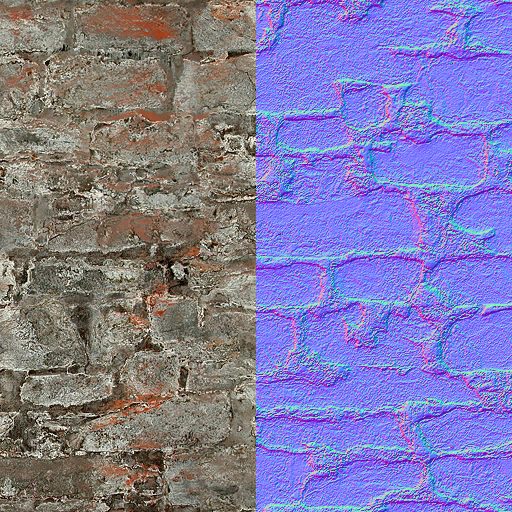
\includegraphics[width=0.33\linewidth]{images/source_texture.jpg}
  }
  \qquad
  \subfloat[\centering in-game]{
    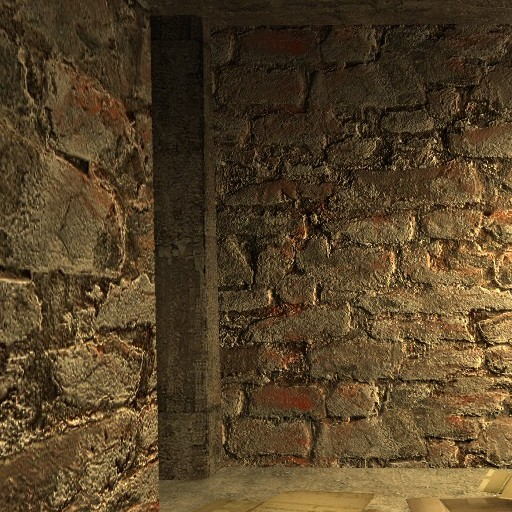
\includegraphics[width=0.33\linewidth]{images/source_texture_game.jpg}
  }
  \caption{The material's textures and in-game appearance}
  \label{fig:source_texture}
\end{figure}

\subsubsection{Unity}
Unity has it's own share of proprietary formats, including but not limited to: animations, curves, gradients, masks, materials, and presets. Unlike Source, Unity uses standard formats for textures and models. It doesn't require models to be compiled, and can even support importing some proprietary model formats (though the \texttt{fbx} format is still preferred). Like Source, Unity supports WAV and MP3 for sounds. However, it additionally supports OGG, FLAC, and some other audio formats.

When Unity assets are imported, the Unity Editor associates some metadata with them. This is used for better integration with the editor. Source doesn't have any notion of importing assets really; Source assets are just loose files or archives with a specific directory structure.

\begin{figure}[!htp]
  \centering
  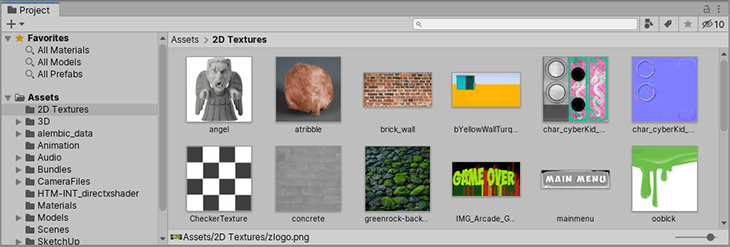
\includegraphics[width=0.75\linewidth]{images/unity_project_window.png}
  \caption{Project window in Unity Editor displaying imported assets}
  \label{fig:unity_project_window}
\end{figure}

Assets can also be bundled into packages which can be imported by other developers. These packages can be put (or sold) on the Unity Asset Store. The Asset Store is not just limited to textures, models, sounds, and even entire scenes. It can provide project templates, scripting tools, visual effects, and much more. This is a major difference from Source, which doesn't have any strong, centralised ecosystem around assets. Thus, a Unity developer is much less reliant on asset creation skills than a Source developer.

Some of Unity's assets are more integrated into the Unity Editor, which makes a developer less reliant on external asset creation. For example, materials in Unity can be directly created in the editor, unlike Source, which requires editing a text file and typing in commands.

\begin{figure}[!htp]
  \centering
  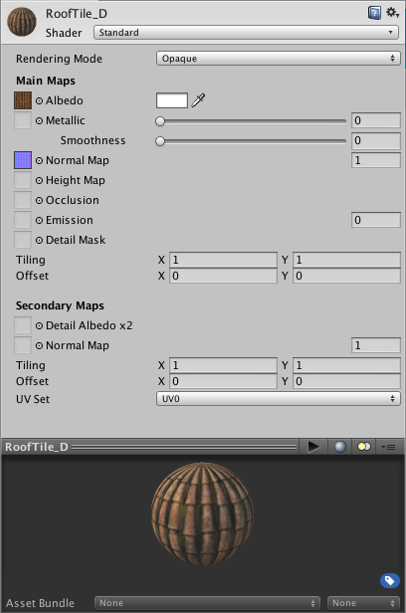
\includegraphics[scale=0.75]{images/unity_material.png}
  \caption{Inspector in Unity Editor showing a material}
  \label{fig:unity_material}
\end{figure}

\subsection{Physics}
\subsubsection{Source}
The Source engine has two 3D physics simulation engines. One is \textit{QPhysics}, which is an older and simpler simulator used for objects with simple collision boxes. It is also used for players, walking NPCs. The more sophisticated engine, \textit{VPhysics}, is not used for them because the simulations would be too complex to handle. VPhysics is based on physics middleware licensed by Havok. It simulates mass, gravity, friction, air resistance, inertia, and buoyancy.

\paragraph{VPhysics}
VPhysics does not use a model's mesh directly for physics simulation. Instead, it uses a collision model, which is typically loaded from the collision mesh of the entity's model. The collision meshes are simpler approximations of the model. Alternatively, collision models can be generated from bounding boxes, which are typically used to perform cheap collision tests.

\begin{figure}[!htp]
  \centering
  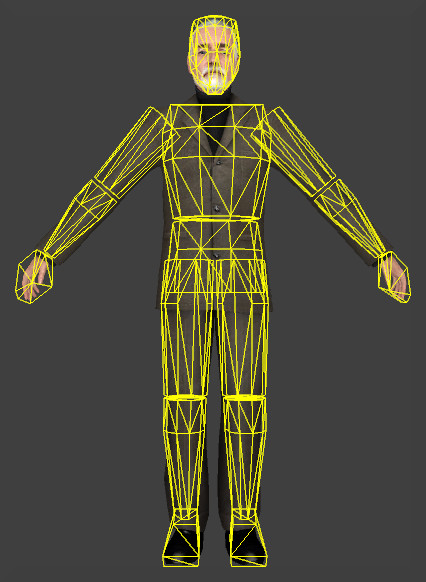
\includegraphics[scale=0.25]{images/source_collision_mesh.png}
  \caption{An NPC's collision mesh}
  \label{fig:source_collision}
\end{figure}

VPhysics-enabled entities have their motion and behaviour influenced by the application of forces and constraints in the world. There are many pre-existing entities for physics which can be used by level designers in Hammer. For example, \texttt{phys\_pulleyconstraint} to simulate a pulley or a \texttt{phys\_hinge} to simulate a hinge. For props, \texttt{prop\_physics} can be used to place a VPhysics-enabled model in the world.

\begin{figure}[!htp]
  \begin{minted}[
    linenos,
    autogobble=true,
    fontsize=\fontsize{10}{10},
  ]{cpp}
    #define MODEL "models/props_c17/FurnitureDresser001a.mdl"

    void CMyEnt::Spawn() {
      PrecacheModel(MODEL);
      SetModel(MODEL);
      VPhysicsInitNormal(SOLID_VPHYSICS, 0, false);
    }
  \end{minted}
  \caption{Programmatically creating a physically-simulated entity}
  \label{fig:source_physics_ent}
\end{figure}

\subsubsection{Unity}

\subsection{Graphics}
\subsubsection{Source}
\subsubsection{Unity}

\subsection{AI}
\subsubsection{Source}
The Source engine has a sophisticated AI system. This system is separate from its choreography system, which won't be part of the discussion. Like all entities, NPCs have a \texttt{Think} function which allows the NPC to schedule code to run in the future. Thinks can be continuously rescheduled to effectively make an entity autonomous. Every time an NPC thinks to make a decision, it follows these steps:

\begin{enumerate}
  \item Perform sensing
  \item Generate a list of conditions
  \item Choose an appropriate state
  \item Selected a new schedule if appropriate
  \item Perform the current task
\end{enumerate}

\paragraph{Sensing}
Sensing is the process of generating a list of entities that an NPC can see and a list of sounds it can hear. These can be filtered out to ignore sights and sounds the NPC shouldn't care about.

An NPC has a potentially visible set (PVS), which is the spatial area that may be visible to the NPC at its current location. When an entity enters the PVS, there a viewcone test is performed to more accurately determine if the NPC can see this entity. The viewcone represents the spatial geometry of the NPC's current visual field, which is determined by the NPC's range (the viewcone's ``depth'') and its field of view (the viewcone's ``scope''). If an entity is within the viewcone, then a line-of-sight test is performed by casting a ray from the NPC to the entity. This determines if the view of the entity is obstructed by another object.

Similar to the PVS, there is a potentially audible set, which is the spatial area that may be audible to the NPC. However, unlike the PVS, there are no further steps involving the viewcone or LOS.

\paragraph{Conditions}
Conditions are flags stored on the NPC which represent some state in the world. They are determined from the sensed sights and sounds. For example, a condition may be set for when an enemy is seen, or when the NPC goes underwater. Conditions can also be used to interrupt schedules. For example, if a condition is set for choosing a new enemy, then this will interrupt a running schedule for chasing the current enemy.

\paragraph{State}
An NPC's state is based upon its conditions. In a sense, a state itself can be thought of as a condition, but in a much broader sense. However, an NPC can only be in one state. Examples of states include being dead, being in combat, and being idle.

\paragraph{Schedule}
The state, together with the conditions, are used to determine an appropriate schedule for the NPC. A schedule is a list of tasks for the NPC to perform, so it can be thought of as an overall action which the NPC is carrying out. An example of a schedule is an NPC taking cover to reload their weapon. An NPC can only have one schedule, and a new schedule is only chosen when there is no active one (due to the previous schedule being completed, failed, or interrupted).

\paragraph{Tasks}
A task is a discrete action within a schedule. Tasks are performed serially until the schedule is completed. Following the example schedule of taking cover to reload, the following tasks would be performed:

\begin{enumerate}
  \item Find a location for cover
  \item Find a path to that location
  \item Traverse the path
  \item Reload the gun
\end{enumerate}

\paragraph{Behaviours}
Behaviours are an abstraction of AI code. They can be re-used by many NPCs rather than being coupled to a single type of NPC. Some pre-existing behaviours include following another NPC, leading the player to a location, or appearing to be ``busy'' (performing some inconsequential action or idling).

\paragraph{Navigation}
NPCs can navigate via a node graph or via a navigation mesh. Typically, the latter is used by ``bots'', though there is a more general-purpose \textit{NextBot} system in some of Valve's games which makes use of navigation meshes. However, it is not available in any public Source SDK release. A navigation mesh can be auto-generated and also manually edited in-game. In contrast, a node graph is generated from manually placed node entities within a map.

\begin{figure}[!htp]
  \centering
  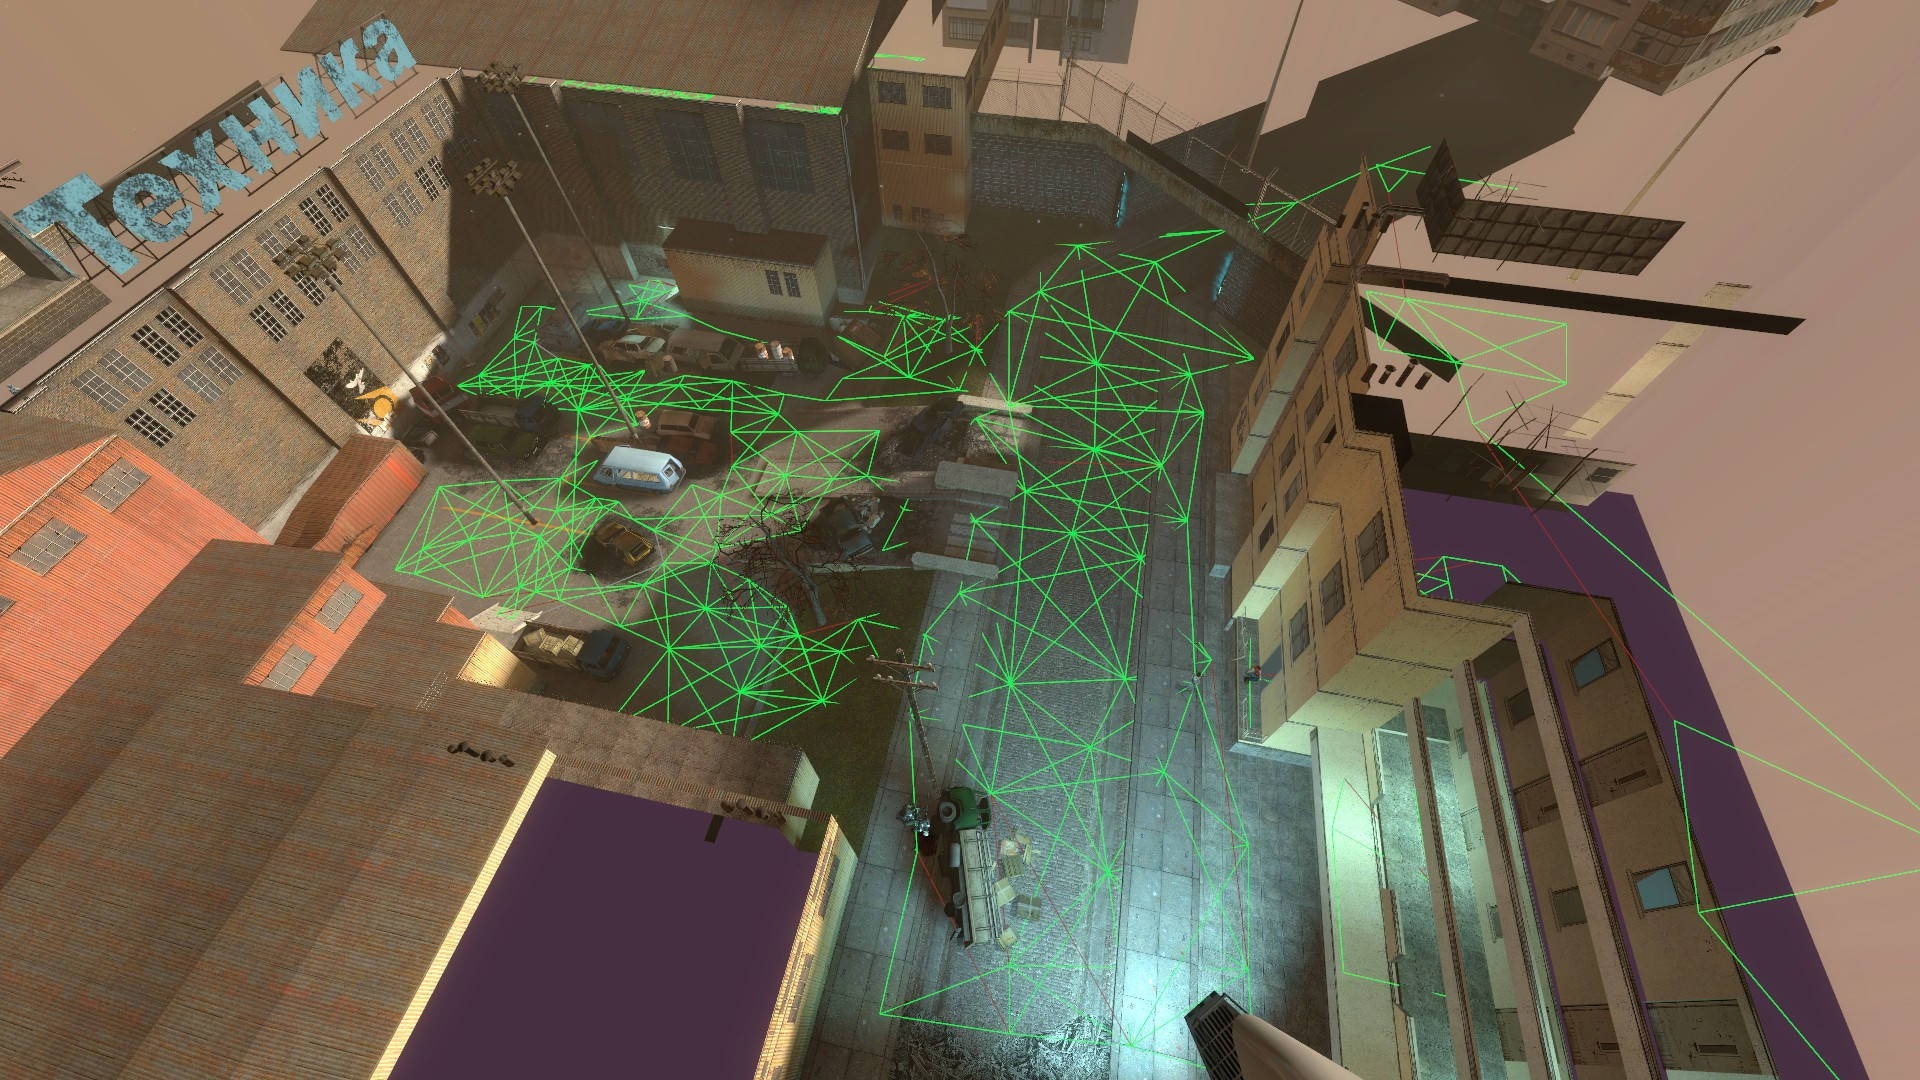
\includegraphics[width=\linewidth]{images/source_node_graph.jpg}
  \caption{A node graph in the penultimate map of Half-Life 2: Episode One}
  \label{fig:source_node_graph}
\end{figure}

\begin{figure}[!htp]
  \centering
  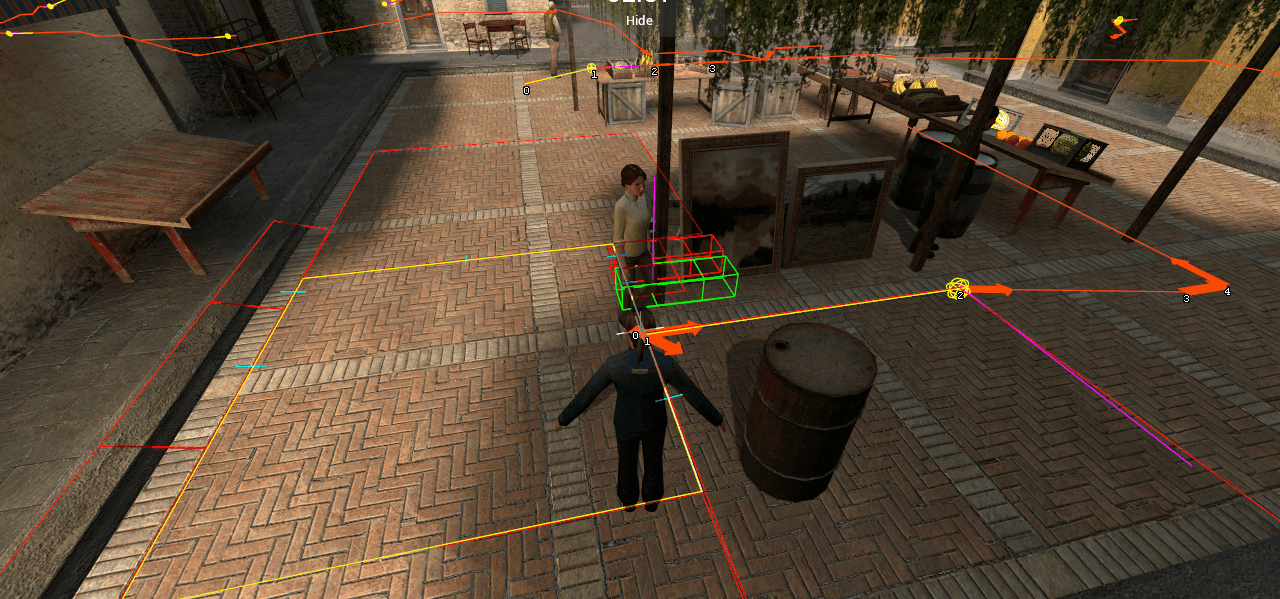
\includegraphics[width=\linewidth]{images/source_nav_mesh.png}
  \caption{Editing a navigation mesh in-game}
  \label{fig:source_nav_mesh}
\end{figure}

\paragraph{Other Features}
There are many other features in the AI system. There is an entire response system to manage speech and dialogue. NPCs can be in squads, which allows them to cover each other, move as a unit, share information, etc. Squads or single NPCs can also be programmed to perform an assault, in which they rally to points and, on cue, commence an assault on one or more points in the world. An NPC can have a relationship with another NPC, such as liking, fearing, or hating another NPCs. For example, if an NPC is fearful of another, they may flee or take cover from them.

\subsubsection{Unity}
Unlike the Source engine, Unity has few AI features inherently. It has an AI module, but it only supports path finding features using a navigation mesh. Other core features such as dialogue or behaviour need to be programmed from scratch, or implemented via a third-party package, such as PandasBT for behaviour trees or Pixel Crusher's dialogue system.

Like with Source, navigation meshes can be automatically generated in Unity. These meshes are the primary way for all path finding, unlike Source which additionally has node graphs.

\begin{figure}[!htp]
  \centering
  \includesvg[inkscapelatex=false, width=0.75\linewidth]{images/unity_nav_loop.svg}
  \caption{Overview of pathfinding in Unity}
  \label{fig:unity_nav_loop}
\end{figure}

\subsection{Networking}
\subsubsection{Source}
Source uses a client-server architecture. The server is typically the authoritative source about the simulation of the world/physics, game rules, and input processing. A client and server communicate with each other using UDP packets. The server sends the world state to clients, and clients base their video and audio outputs on this received state. Clients receive inputs from players and send that data to the server for processing.

The game is simulate by the server in discrete units of time called \textit{ticks}. For each tick, the server processes inputs, runs a step of the physics simulation, checks game rules, and updates object states. By default, the tick rate is $66.\bar6$ ticks per second. This can be increased to make the simulation more precise, but at the cost on increase CPU and bandwidth usage.

After simulation, the server determines if there are clients in need of a world update, and if so, it generates a snapshot of the current state to later send to the clients. These snapshots are used instead of sending a new update packet to each client for every change. The server employs \textit{delta compression} for these snapshots to avoid sending redundant information. The idea is to only send a snapshot including the states that actually changed. To achieve this, the client must acknowledge the updates it receives. The server generates the delta snapshot based on the updates that have occurred since the last acknowledged update by the client. In cases of packet loss, full snapshots may be sent to clients to help them recover.

Similar to the server's snapshots, the client does not send a packet for every user command (user inputs). Instead, it groups commands together and sends them in a single packet at a fixed rate.

\paragraph{Interpolation}
To conserve bandwidth, snapshots are sent at a rate of 20 per second by default. This is not sufficient for the clients to render the updates smoothly. To avoid a choppy appearance, the client interpolates entity state between the two most recent snapshots. At 20 snapshots per second, a new snapshot arrives every 50 milliseconds. Thus, the client has to interpolate the last 50 milliseconds to make things appear smooth.

Packet loss can have a detrimental effect on interpolation. To solve this, the interpolation period is set to 100 milliseconds by default. This means that if the previous snapshot is lost, the one before it will still be within the period for interpolation. \cref{fig:source_net_interp} demonstrates this: even if the snapshot at tick 342 is lost, the snapshot at 340 is still within the interpolation period. This does effectively mean that the client's view is always behind by 100 ms, or whatever the configured period is.

\begin{figure}[!htp]
  \centering
  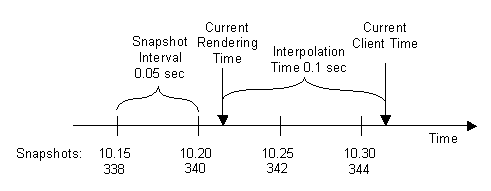
\includegraphics[width=0.66\linewidth]{images/source_net_interp.png}
  \caption{Interpolation timeline with a period of 100 ms}
  \label{fig:source_net_interp}
\end{figure}

Of course, a leeway of 2 snapshots isn't always sufficient; both snapshots could be lost. In such cases, the client can linearly extrapolate state based on the client's last known state of that entity. However, this is only done up to a certain duration of packet loss; beyond that, prediction errors are too severe.

\paragraph{Prediction}
Clients inevitably have some network latency. If the client had to strictly rely on the server for updates resulting from player input, the visual feedback to the player would be delayed by the network latency. Client-side prediction solves this by predicting and rendering the results of the player's inputs without waiting for the server. This only affects the client's view; the server will still consider the client to be in the previous state until it receives the user command packet.

When the client finally receives the snapshot from the server, it will compare its own state to the server's. A prediction error occurs if these states do not match. In such case, the client has to correct the error, since the server is the authority. To make the errors less noticeable, the prediction error smoothing is used to gradually move to the server's state.

\paragraph{Lag Compensation}
Due to variations in latency, clients don't always all have their states in-sync with each other and with the server. This results in consistencies between clients. A scenario may occur where an attacking player shoots a target player, but the attacker had higher latency. The target may have moved out of harm's way, but the attacker did not receive that update yet at the time of the shot being fired. Thus, to the attacker, it appears as though the target should be hit, but the server would not consider it a hit since it's the authority on the positions of players and the attacker's client was out of date.

To solve this inconsistency, the server uses lag compensation. When a user command (such as a fired shot) is received, the server estimates at what time that command was created. It has to account for latency and interpolation on the client. Using a short history of player positions, the server simulates the positions of the players at the estimated time of the command's execution. It then uses these positions to process the input.

The server will realise that at the time the attacker shot, the target was actually in line with the shot. Thus, it will register the hit. Afterwards, the simulation will revert players to their actual positions. This isn't perfect, since it results in anomalies such as the target being hit even though to them, they are already behind cover. Such consequences are generally unavoidable, but in practice, packet speeds are sufficiently quick to avoid these sorts of problems.

\begin{figure}[!htp]
  \centering
  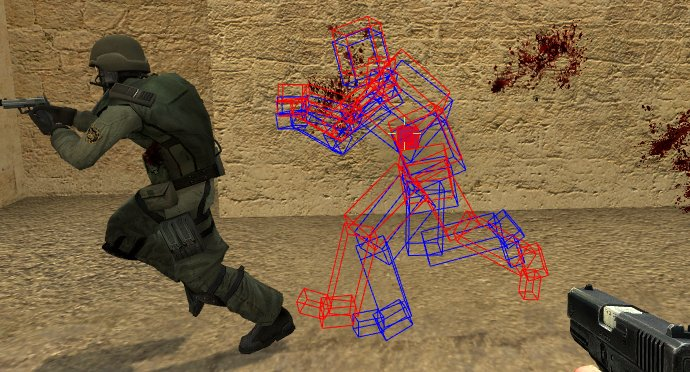
\includegraphics[width=0.66\linewidth]{images/source_net_lag_comp.jpg}
  \caption{Lag compensation}
  \label{fig:source_net_lag_comp}
\end{figure}

In \cref{fig:source_net_lag_comp}, 200 milliseconds of lag is being faked by the client. The red hitbox is the position on the client at the time of the shot. The blue hitbox is the server's position based its the estimated time of the shot. The two hitboxes don't perfectly line up due to precision errors in estimate the command's time. However, they are still close enough for the server to successfully register the shot as a hit.

\paragraph{Networking Entities}
Both logical and physical objects in the world are called \textit{entities}. There are client-only entities, sever-only entities, and entities which are on both sides. The engine is responsible for ensuring these entities remain in sync. It does this through snapshot packets, which were discussed earlier.

Going into more detail, the engine has to detect changes in the server-side entity, serialise the changes, send that as a network packet, deserialise it on the client, and update the corresponding client-side entity.

An entity is a class that inherits from \texttt{CBaseEntity}. Entities that need to be synchronised between the client and server are assigned indices which are tracked by an \textit{entity dictionary} to ensure the indices are consistent on both sides. Not all member variables of the entity class need to be sent over the network. The ones that should be networked are designated using \texttt{CNetworkVar} and other similar macros (there are variations for other data types).

\begin{figure}[!htp]
  \begin{minted}[
    linenos,
    autogobble=true,
    fontsize=\fontsize{10}{10},
  ]{cpp}
    CNetworkVar(int, m_iMyInt);
    CNetworkVar(float, m_fMyFloat);
    CNetworkVector(m_vecMyVector);
    CNetworkQAngle(m_angMyAngle);
    CNetworkArray(int, m_iMyArray, 64);
    CNetworkHandle(CBaseEntity, m_hMyEntity);
    CNetworkString(m_szMyString);
  \end{minted}
  \caption{Declared network variables}
  \label{fig:source_net_var}
\end{figure}

Snapshot update packets are built from serialised network variables. Thus, entity classes must define how their networked variables are serialised and deserialised. This is done with \textit{data tables}. \textit{Send tables} are for serialisation and \textit{receive tables} are for deserialisation. Each network variable's serialisation or deserialisation information is stored in the data table as a \texttt{SendProp} or \texttt{RecvProp}, respectively.

\begin{figure}[!htp]
  \begin{minted}[
    linenos,
    autogobble=true,
    fontsize=\fontsize{10}{10},
  ]{cpp}
    IMPLEMENT_SERVERCLASS_ST(CMyClass, DT_MyClass)
        SendPropInt(SENDINFO(m_iMyInt), 4, SPROP_UNSIGNED),
        SendPropFloat(SENDINFO(m_fMyFloat), -1, SPROP_COORD),
        SendPropVector(SENDINFO(m_vecMyVector), -1, SPROP_COORD),
        SendPropQAngles(SENDINFO(m_angMyAngle), 13, SPROP_CHANGES_OFTEN),
        SendPropArray3(
            SENDINFO_ARRAY3(m_iMyArray),
            SendPropInt(SENDINFO_ARRAY(m_iMyArray), 10, SPROP_UNSIGNED)
        ),
        SendPropEHandle(SENDINFO(m_hMyEntity)),
        SendPropString(SENDINFO(m_szMyString)),
    END_SEND_TABLE()
  \end{minted}
  \caption{Declared send table}
  \label{fig:source_net_send_table}
\end{figure}

\subsubsection{Unity}
There are several networking APIs offered by Unity. First is the now deprecated UNet, which houses the high-level networking API (HLAPI) and the Transport Layer API. The latter is a lower-level API meant for more advanced multiplayer games. Unity is also working on a new multiplayer and networking solution named \textit{Netcode for GameObjects}. This is meant to replace UNet.

\begin{figure}[!htp]
  \centering
  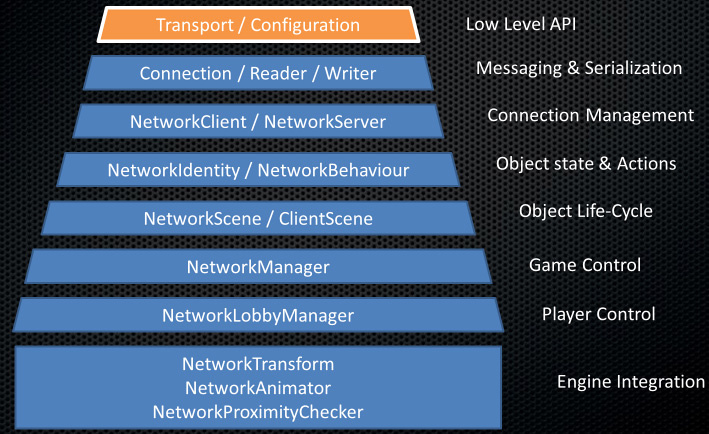
\includegraphics[width=0.66\linewidth]{images/unity_net_layers.png}
  \caption{Layers of the HLAPI}
  \label{fig:unity_net_layers}
\end{figure}

Akin to network entities in Source, there is a Network Identity component that makes game objects uniquely identifiable across the client-server boundary. Also like Source, Unity can automatically synchronise the states of game objects and script variables. This is done through various components, such as Network Transforms for position synchronisation and Network Animators for animation synchronisation. This component-based system, which is fundamental to Unity as a whole, is quite different from how synchronisation is defined in Source.

Fields of scripts can be synchronised using \texttt{SyncVar} annotations. This is more similar to the macros used in Source to designate variables as networked. As with source, this kind of synchronisation is uni-directional; data is synchronised from the server to remote clients. To perform synchronisation in the opposite direction in Unity, commands have to be used. This is also similar to Source, which has the client send user command packets to the server.

\begin{figure}[!htp]
  \centering
  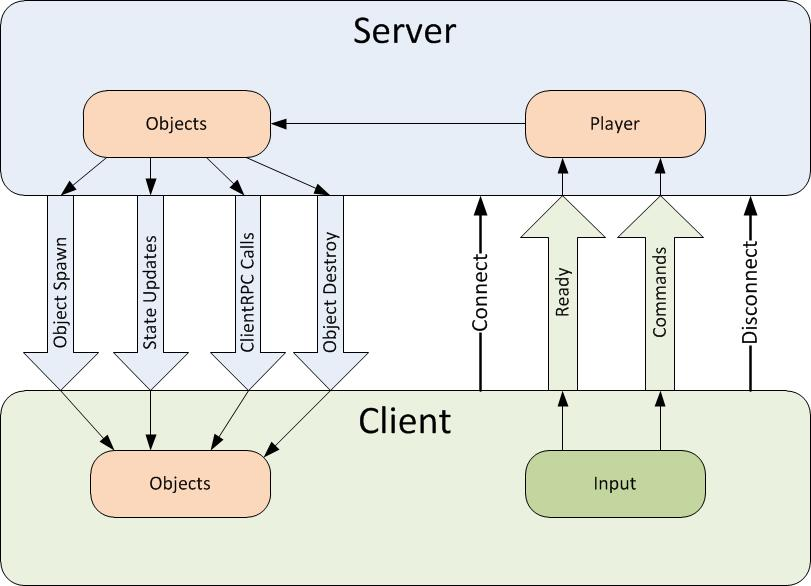
\includegraphics[width=0.66\linewidth]{images/unity_net_actions.jpg}
  \caption{Directions of remote actions}
  \label{fig:unity_net_actions}
\end{figure}

\paragraph{Lag}
UNet can support interpolation like Source. However, client-side prediction and lag compensation seem to only be features supported by the newer Netcode for GameObjects. These concepts are standard in the industry, so Unity's implementation of them isn't too dissimilar to Source's. Netcode also supports \textit{action anticipation}, which is similar to client-side prediction, but more restrictive. The example used to explain it is a grenade throw. It shouldn't be fully predicted on the client side since its destructive abilities may cause prediction errors which are too noticeable. In such case, it may be desirable to play non-gameplay impacting animations, sounds, and effects while still relying on the server to confirm the grenade's trajectory and destructive consequences.

\subsection{Platforms}
\subsubsection{Source}
The Source Engine can target the PC (Windows, macOS, and Linux), Xbox 360, and PlayStation 3. Originally it only supported Windows. Xbox 360 and PlayStation 3 support came with the Source 2007 branch of the engine, which was released alongside the \textit{Orange Box}. Mac OS X support was added in the Source 2009 branch. Linux support came in the Source 2013 branch, though it was at least possible to compile a game server for Linux in earlier versions too.

\subsubsection{Unity}
Unity supports many more platforms than the Source Engine. Source's console support is quite dated at this point, and it has no extended reality or mobile support. Unity supports the following platforms:

\begin{itemize}
  \item Desktop
  \begin{itemize}
    \item Windows
    \item Mac
    \item UWP
    \item Linux
  \end{itemize}
  \item Mobile
  \begin{itemize}
    \item iOS
    \item Android
  \end{itemize}
  \item Extended Reality
  \begin{itemize}
    \item ARKit
    \item ARCore
    \item Microsoft HoloLens
    \item Magic Leap (Lumin)
    \item Oculus
    \item PlayStation VR
  \end{itemize}
  \item Consoles
  \begin{itemize}
    \item PS5
    \item PS4
    \item Xbox One
    \item Xbox X|S
    \item Nintendo Switch
    \item Google Stadia
  \end{itemize}
  \item WebGL
\end{itemize}

\begin{figure}[!htp]
  \centering
  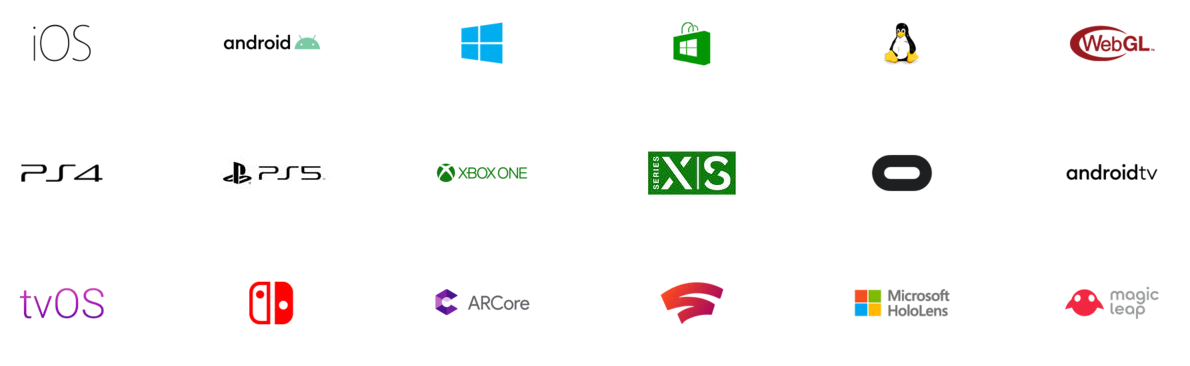
\includegraphics[width=\linewidth]{images/unity_platforms.png}
  \caption{Some of Unity's supported platforms}
  \label{fig:unity_platforms}
\end{figure}

The Unity engine has been around since 2005, so there are many outdated platforms it used to support. For example, it used to support the Wii, Xbox 360, BlackBerry 10, and Windows Phone 8.

In general, Unity has kept up better with release platforms compared to Source. This is because Valve prioritised developing their own games first, so their engine features suited their games' needs. In contrast, Unity isn't a game publisher or studio, so their core product is the engine itself. Valve shifting resources towards the development of Source 2 also contributed to Source 1 falling behind.

\end{document}
